\documentclass[10pt,twocolumn,letterpaper]{article}

\usepackage{3dv}
\usepackage{times}
\usepackage{epsfig}
\usepackage{graphicx}
\usepackage{amsmath}
\usepackage{amssymb}
\usepackage{mathtools}
\usepackage{float}
\usepackage{stfloats}
\usepackage{hyperref}


% Include other packages here, before hyperref.

% If you comment hyperref and then uncomment it, you should delete
% egpaper.aux before re-running latex.  (Or just hit 'q' on the first latex
% run, let it finish, and you should be clear).
%\usepackage[pagebackref=true,breaklinks=true,letterpaper=true,colorlinks,bookmarks=false]{hyperref}

\threedvfinalcopy % *** Uncomment this line for the final submission

\def\threedvPaperID{****} % *** Enter the 3DV Paper ID here
\def\httilde{\mbox{\tt\raisebox{-.5ex}{\symbol{126}}}}

% Pages are numbered in submission mode, and unnumbered in camera-ready
\ifthreedvfinal\pagestyle{empty}\fi
\setcounter{page}{4321}
\usepackage{hyperref}
\usepackage{cleveref}
\begin{document}

%%%%%%%%% TITLE
\title{Event-based Mosaicing and Tracking}

\author{Jo\"el Bachmann\\
D-MAVT, ETH Zurich\\
{\tt\small bajoel@student.ethz.ch}
% For a paper whose authors are all at the same institution,
% omit the following lines up until the closing ``}''.
% Additional authors and addresses can be added with ``\and'',
% just like the second author.
% To save space, use either the email address or home page, not both
\and
Nik Dennler\\
INI, University of Zurich\\
{\tt\small nik.dennler@uzh.ch}
\and
C\'eline Nauer\\
INI, University of Zurich\\
{\tt\small celine.nauer@uzh.ch}
}



\maketitle
%\thispagestyle{empty}

%%%%%%%%% ABSTRACT
\begin{abstract}
Event cameras employ biologically inspired vision sensors which record pixel-level intensity changes. Compared to standard cameras with fixed frame rates, these intensity changes are recorded asynchronously and generate so-called events. 
This working principle leads to advantages such as a very high dynamic range, low latency and no motion blur. 
However, standard computer vision algorithms can not be applied to an event-stream and thus, novel algorithms are needed. In this project, we re-implement the mapping and tracking algorithm proposed by Kim et al. 
The algorithm consists of two parts: a Particle Filtering method for tracking and an Extended Kalman Filter for the intensity map reconstruction. We examine the parts separately on a simulated, noise-free dataset for baseline investigation.
Further, we provide a self-recorded DAVIS dataset and attempt to improve the ground truth poses using ORB-SLAM on image frames. Inspecting the performance of the algorithm on the simulated dataset shows acceptable results, while the recorded dataset was not processed successfully. We conclude that the method is not optimal and would have to be adapted further in order to cope with real data sets.
\end{abstract}




%%%%%%%%% BODY TEXT
\section{Introduction and Problem Statement}

The nature of a dynamic vision sensor lead to favourable performance such as short latency and a high dynamic range. This gives them a large potential for applications in computer vision, robotics and autonomous mobility. Event-based methods are especially promising in settings where traditional cameras fail due to their limitations, for instance high-speed scenarios. By appropriately exploiting the output of these sensors through novel algorithms, a range of unsolved problems in vision could potentially be tackled. 

%-------------------------------------------------------------------------

\subsection{Dynamic Vision Sensor}

\paragraph{Working principle:}
Traditional cameras capture images in frames, such that all pixels are evaluated synchronously at a fixed rate. Event cameras are bio-inspired sensors that work radically different. Each pixel measures the brightness change independently from the others and generate a so-called event, once a brightness threshold is crossed. An event $e$ is the encoding of time $t$, pixel coordinates $(u,v)$ and polarity $p$ of the brightness changes.
\begin{equation}
e(u,v) = (u,v,p,t)
\end{equation}
For each pixel, an event is triggered if the difference of the log intensities is smaller or larger than a camera-specific threshold value $C_{th}$:
\begin{equation}
    \Delta \ln{I} \coloneqq \ln{(t)} - \ln{(t-\Delta t) \gtrless
C_{th} } 
\end{equation}
The output of an event camera is then a stream of asynchronously generated events. 

\paragraph{Characterizing attributes:}
Event cameras possess outstanding properties compared to traditional cameras: very high dynamic range (140 dB vs. 60 dB), low latency (in the order of microseconds), low power consumption (in the order of mW), reduced bandwidth, and virtually no suffering from motion blur \cite{EventVisionReview}.

\paragraph{State-of-the-Art:}
Event cameras are based on the Dynamic Vision Sensor (DVS), which has been developed by D. Lichtsteiner and T. Delbruck in 2008 \cite{DVSoriginal}. It is based on MOSFET technology, in a circuit where most transistors are kept in their sub-threshold range. The succeeding state-of-the-art sensor is called Dynamic and Active Pixel Vision Sensor (DAVIS); it combines the DVS technology with an active pixel sensor (APS). Thus, it outputs events and frames \cite{DAVIS}. A visual summary of DAVIS, including a simplified schematics of the DVS circuit, is shown in \cref{fig:davis}. 

\begin{figure}[h!]
	\centering
    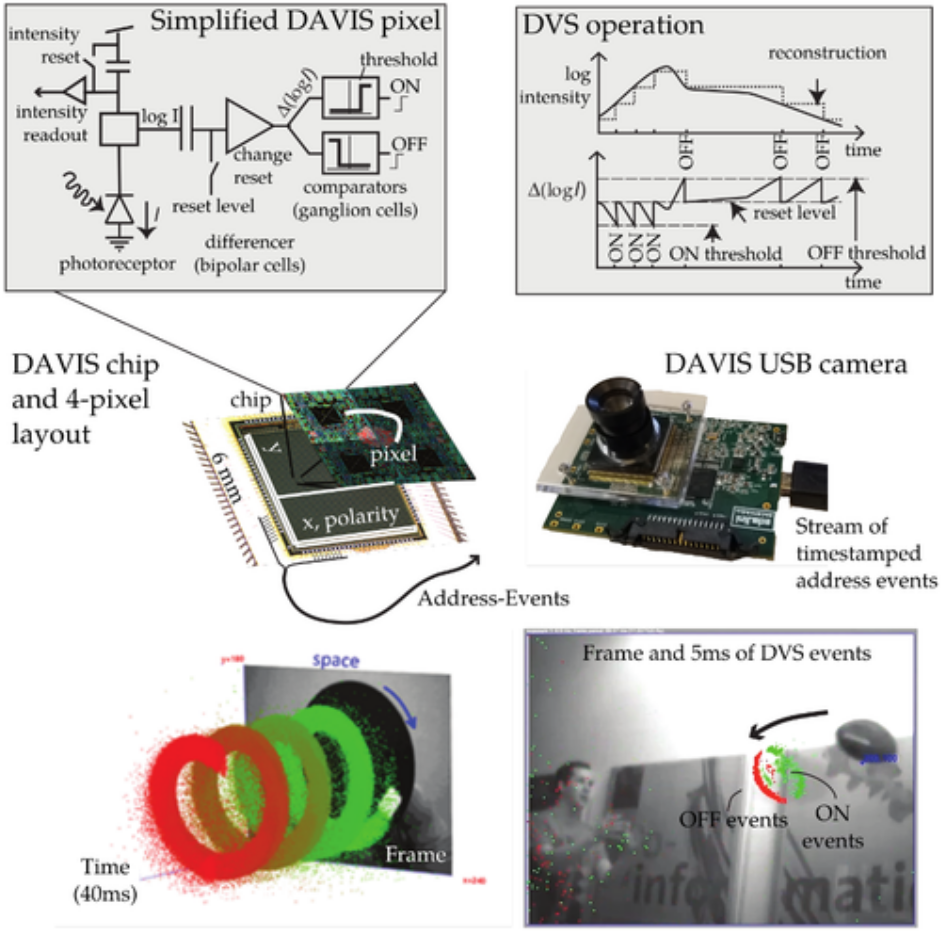
\includegraphics[width=0.99\linewidth]{figures/davis.png}    
    \caption{Wrap-up of the Dynamic and Active Pixel Vision Sensor (DAVIS). \textbf{Top-left:} Simplified DAVIS-pixel circuit. A capacitor is charged by the current flowing through a photo-diode and then read out.  \textbf{Top-right:} Working principle of the DVS. Events are produced if the difference in log-intensity rises or falls below a positive or negative threshold respectively. \textbf{Center:} DAVIS chip and USB camera. \textbf{Bottom-left:} Visualization of positive events (green), negative events (red) events and frames caused by a spinning dot.  \textbf{Bottom-right:} Events super-imposed on frames. Images and description adapted from \cite{EventVisionReview}.}
    \label{fig:davis}
\end{figure}


\subsection{Problem description}
This project aims to re-implement the approach proposed by Kim et al. \cite{kim2014simultaneous} in order to  iteratively create an intensity map of the scene and track the rotational camera pose.
To assess the performance of the method, we propose to apply the algorithm to a simulated dataset and additionally to a self-recorded dataset, using a DAVIS camera. To make the work easy and non-commercially accessible for future projects, we decide to implement the code in Python.


\subsection{Related work}

First attempts at combining the estimation of ego-motion, image intensity and optical flow for rotational movement from an event stream was proposed by \cite{cook}. The first tracking algorithm for event-based cameras was introduced in 2012 by \cite{weikensdorfer}. 
Slow, planar motion is tracked by following the visual stimuli of an artificial B \& W pattern perpendicular to the robots direction of motion. Succeeding this work \cite{mitrgbd} proposes an algorithm for ego-motion tracking of a B&W, planar scene, where a standard gray-scale camera was attached to a DVS. 
A Bayesian Filter is used to process both sensor inputs and estimate the deviance between the current event and the previous frame of the gray-scale camera. 
In a similar way, \cite{weikensdorfer2} combine a depth sensor with a DVS which outputs a sparse stream of events adapted by the depth sensor used for 3D SLAM. The described approaches attempt to solve the problem of 3D ego-motion tracking, however they rely on frame-based techniques and thus are prone to error due to motion blur. Almost simultaneous to the work of Kim et al., \cite{austria} similarly proposed an algorithm for panoramic scene reconstruction for event-based systems. However, their task-specific hardware components restrict adaptation and flexibility to solve other tasks. Their $360^\circ $ high dynamic range camera consists of a stereo setup of DVS mounted on a mechanical rotating device with a processing unit. \\

Based on these preceding projects, \cite{kim2014simultaneous} proposes a pioneering solution for tracking and mapping in a rotational setting and acted as a building block for a number of follow-up papers in intensity reconstruction as well as simultaneous localization and mapping (SLAM) with event cameras. Succeeding \cite{kim2014simultaneous}, \cite{reinbacher} shows the simultaneous tracking and intensity reconstruction in 6 DoF. Following this, numerous projects have extended the previously proposed tracking and mapping methods in event-based SLAM such as \cite{paperpresentation} and even Star-tracking algorithms \cite{startracking}.


\section{Algorithm}
The algorithm which was implemented in this project is based on the theoretical framework of \cite{kim2014simultaneous}. As shown in \cref{fig:algorithm}, the method consists of two alternating steps. 

\begin{figure}[h!]
    \centering
    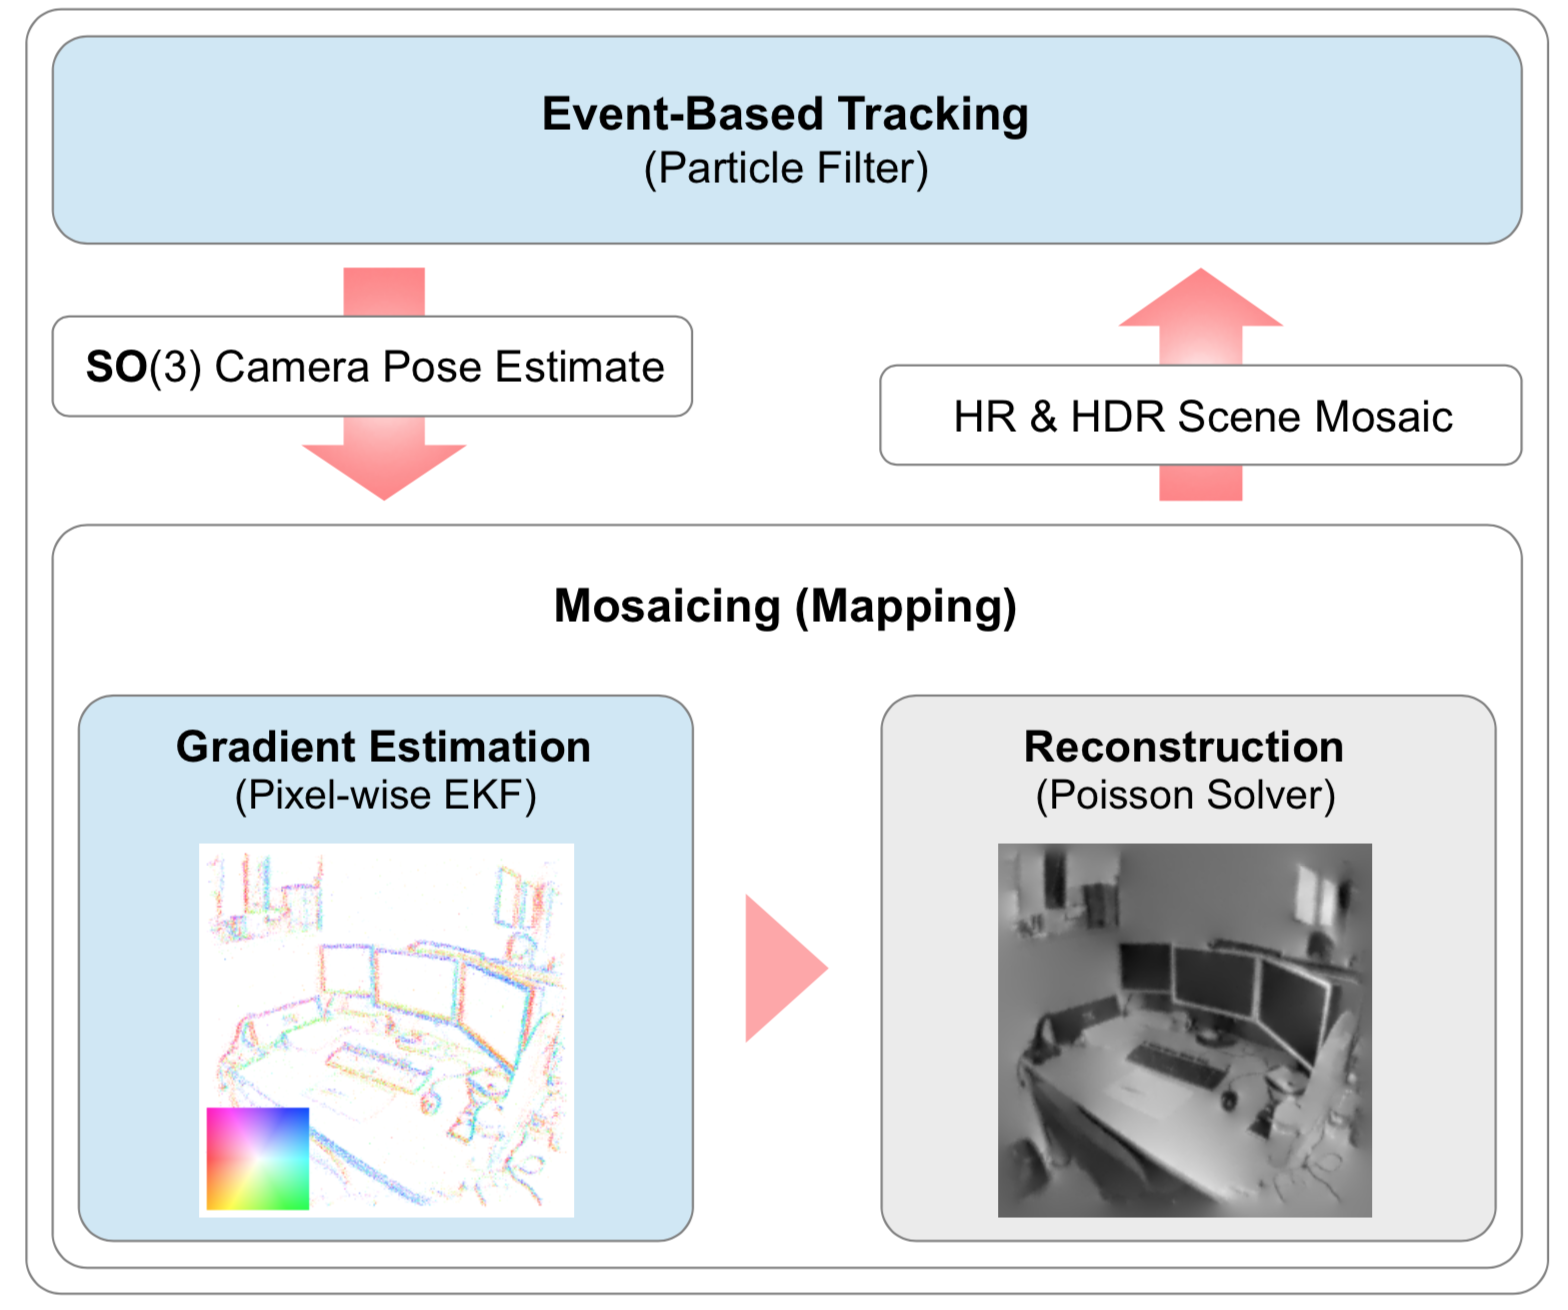
\includegraphics[width=0.5\textwidth]{figures/algo.png}
    \label{fig:algorithm}
    \caption{Schematic overview of the algorithm proposed by \cite{kim2014simultaneous}. The following parts are iteratively executed: A tracking method implemented with a Particle Filter to estimate the rotational pose of the camera (top), an Extended Kalman Filter to update the gradient map of the scene (bottom left) and a Poisson solver to generate the intensity map of the scene (bottom right).}
\end{figure}

First, the "event-based tracking" translates events and an existing mosaic into SO(3) camera pose estimates. Then, the "mosaicing" takes poses and events as input and updates the intensity map. In the following, the subparts of the proposed algorithm are explained in detail. 

\subsection{Particle Filter for Tracking of the Camera Pose}
A Particle Filter is a probabilistic approach of Bayesian Filtering, where the pose of the sensor is approximated by $N$ particles. 
Each particle is a tuple $(R_i, w)$ consisting of a $3\times 3 $ rotation matrix $R_i$ and a corresponding likelihood $w_i$.
A Particle Filter iterates between two main steps:
\subsubsection*{Motion Update}
In the update step, each particle $(R_i, w)$ is updated according to a function describing the development of the state. Since our algorithm should work with any movement of the DVS, the particles are randomly scattered according to a normal distribution around all degrees of freedom. To consider the velocity of the movement, we choose the variance to be proportional to the density of events over time for the current batch. Thus, the updated particle is given as 

\begin{equation}
      R^{(t)}_i = R^{(t-1)}_i \exp \left(
    \sum_{k=1}^3n_k G_k
    \right) \\
\end{equation}
where $G_k$ are the generators of SO(3) and $n_k$ is given as 

\begin{equation}
    n_k \sim \mathcal N (0, \sigma_i^2\tau).\\
\end{equation}


\subsubsection*{Measurement}
The goal of the measurement step is to assign a likelihood to all particles. In essence, we take each particle and evaluate how likely the corresponding pose is compared to the event that occurred. 
In our case, the measurement $z$ is the log intensity difference between the corresponding intensity map positions. 
As each event contains a polarity ($\pm 1$), we can - for each pair of events in a step on the intensity map - deduce its polarity. If the polarity of the event doesn't match the pose change on the intensity map, we assign a low likelihood. All other events are weighted according to a mexican-hat-shaped likelihood curve, which represents the sensor model of the camera (see \cref{fig:mexican}). 

\begin{figure}[h!]
   \centering
    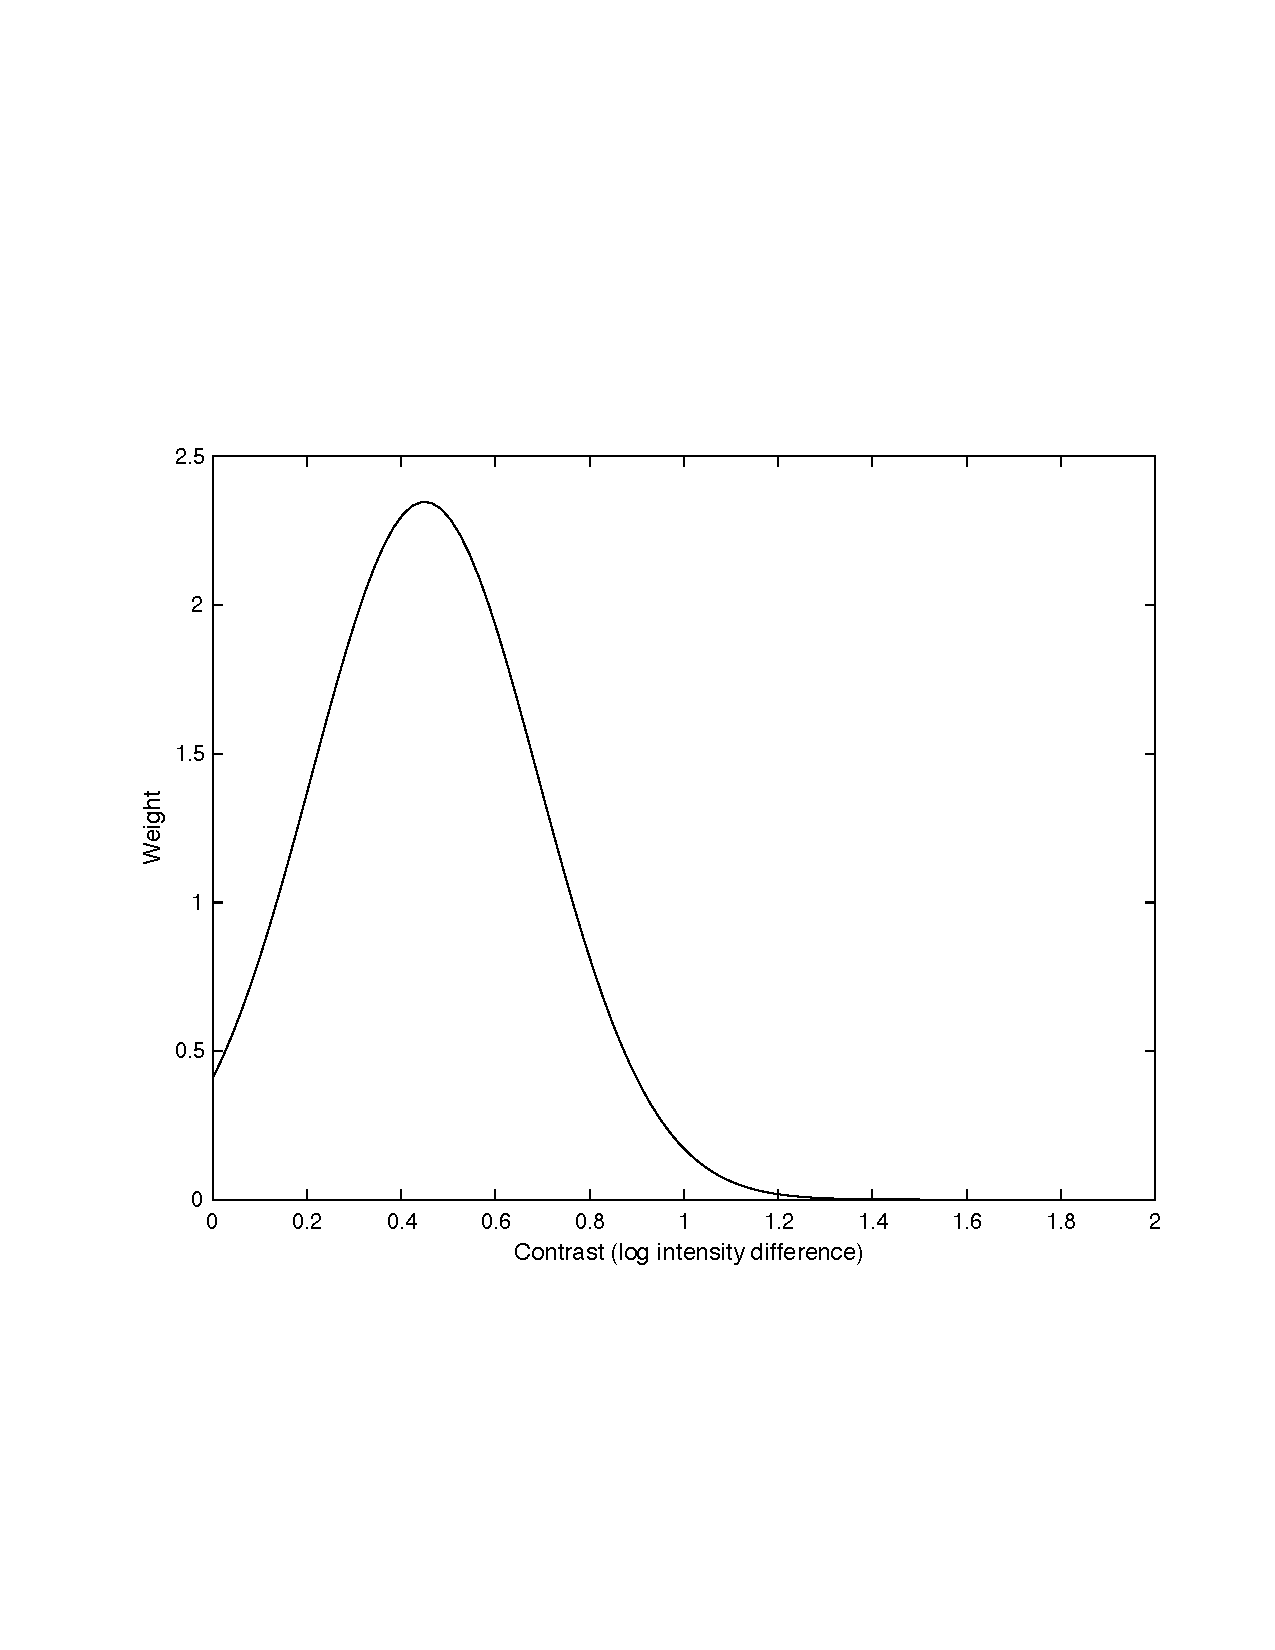
\includegraphics[width=0.6\linewidth]{figures/mexican.pdf}
    \label{fig:mexican}
    \caption{Mexican-hat likelihood function. The weight of each particle is determined by applying the function to the difference in log intensity for two succeeding events at the same pixel. The center and the spread of the curve is specific to the sensor model of the camera.\cite{kim2014simultaneous}}
\end{figure}

The resulting weights are normalized and the particles are re-sampled accordingly. This results in $N$ particles contained in a subset of the sampled particles, all with equal weights. These are then averaged in order to get an estimate of the sensor pose, that can be passed to the intensity reconstruction.

\subsection{Mosaicing}
The goal of mosaicing is to generate an intensity map from the poses and the event stream. This is done in two steps, as seen in Fig. \ref{fig:algorithm}.
First, a pixel-wise Extended Kalman Filter (EKF) assigns a gradient to each pixel on the $1024 \times 2048$ map. Then, using a Poisson Solver, we use these gradients to approximate the intensity map.

\subsubsection*{EKF Estimation}
With an estimate of the state and a stream of events, it is possible to project each event onto the intensity map using the intrinsic calibration of the event-based camera. We denote an event at time $t$ as $e^{(t)}(u,v)$. $\tau$ is the pixel-specific time difference between two events on the same pixel. Projecting $e^{(t)}(u,v)$ and $e^{(t-\tau)}(u,v)$ onto the map, we know the gradient change between those two points. We then find the midpoint between those points, and update its log intensity gradient with the direction of the movement. 
This way, each  new event improves the previous estimate of the gradient map.

\subsubsection*{Poisson Reconstruction}
We now want to generate an intensity map from the gradient map generated from the EKF in the previous step. Since the vector field is not integrable, it is not possible to simply integrate the gradients to receive an intensity map. Therefore, a Poisson Solver is implemented, which generates an intensity map by minimizing the squared difference between the gradients of the intensity map and the gradient map  \cite{kim2014simultaneous}. 
$$
\min \int \int \left( \frac{\partial M_l}{\partial x}-g_x  \right)^2 +
\left(\frac{\partial M_l}{\partial x}-g_x
\right)^2 dxdy
$$
Here, $g_x$ and $g_y$ denote the pixel-wise gradient in $x$ and $y$ direction respectively and $M_l$ is the log intensity map.

%\newpage
\section{Datasets}
The proposed algorithm was evaluated on the following two types of datasets: 
\subsection{Simulated dataset}

From RPG at University of Zurich, we obtained a dataset that has been generated with an event-simulator as deployed in \cite{simulator}. Based on the measurement model of a DAVIS, given a virtual 3D scene and the trajectory of the camera, the simulator generates the DVS event-stream, the respective APS intensity frames and the ground-truth camera poses in units of quaternions. Although highly complex, the generated dataset is noise-free and thus should offer a good estimate for the ideal performance of the algorithm. 

\subsection{Recorded Dataset}
Using a DAVIS348, we recorded multiple datasets and evaluated their quality regarding complexity of the scene, noisiness of the event stream and illumination of the standard camera. We decide on a set with a low scene complexity, high and uniform illumination and a long measurement duration (approx. 30s). 
The dataset includes the DVS events, the APS frames and the IMU data. The recording of the dataset and the camera calibration was performed with the ROS driver and checkerboard-calibration tool of the RPG group \footnote{See \url{https://github.com/uzh-rpg/rpg_dvs_ros}} as shown in \cref{fig:recording}. 
 
\begin{figure}[h!]
    \centering
    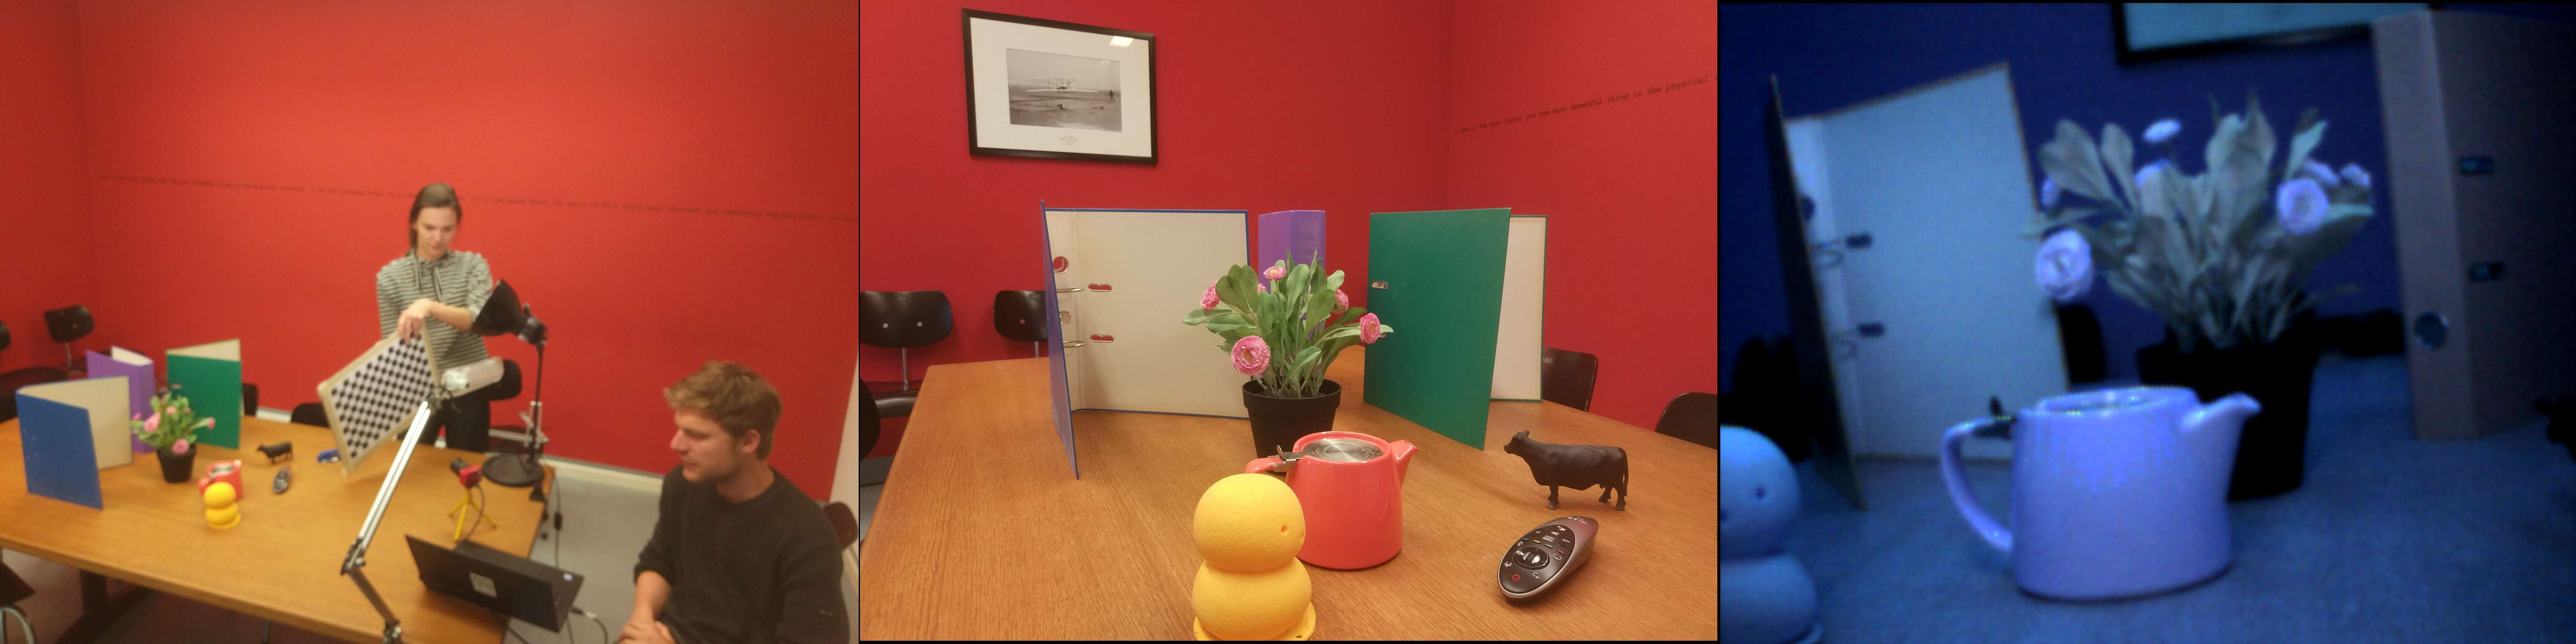
\includegraphics[width=1.0\linewidth]{figures/dataset_recording3.jpg}
        \caption{Capturing our own dataset. \textbf{left:} Objects of various shapes and sizes are placed at different depths. Different lamps are used to illuminate the scene optimally. The camera is calibrated using the checkerboard method. The recording is done with a conventional laptop and the ROS framework. \textbf{center:} Sideways view on the resulting scene. \textbf{right:} A part of the resulting scene as perceived with DAVIS.}
    \label{fig:recording}
\end{figure}


\section{Results}
\subsection{Simulated Dataset}
First we run the reconstruction and tracking algorithm on the simulated dataset created by the event generator. To tackle the problem of simultaneous mosaicing and tracking, we choose a modular approach and build and execute both parts seperately. First, the reconstruction was done based on the event stream and the ground truth poses. 

\subsubsection{Mosaicing}
The Extended Kalman Filter outputs the gradient maps in $x$ and $y$, which are then fed into a Poisson solver to get the final image reconstruction. Both the gradient maps and the reconstructed image of the scene are shown in \cref{fig:reconstruction_simulated}. 

\begin{figure}[h!]
	\centering
    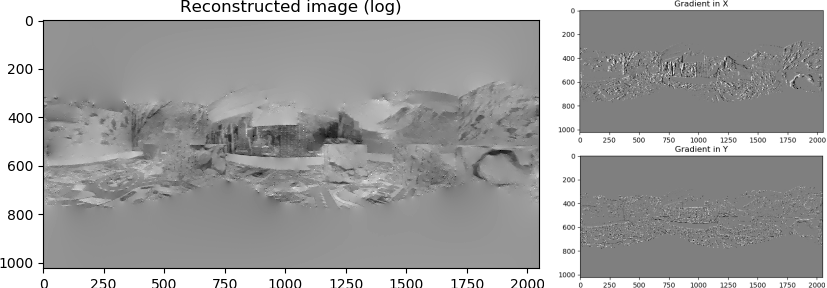
\includegraphics[width=1.0\linewidth]{figures/reconstructed_and_gradient.png}   \caption{Reconstruction from simulated dataset. \textbf{left:} Reconstructed image of the simulated scene after Poisson solver is applied to gradient maps. \textbf{right:} Gradient maps in x and y respectively.}
    \label{fig:reconstruction_simulated}
\end{figure}

We observe that the reconstruction adequately reproduces the scene. The features are already observable in the gradient maps. In the reconstructed image, the scene details are clearly visible and there is almost no ghosting or shadowing apparent. 

\subsubsection{Tracking}
The output of the reconstruction was then used as the ground truth for the tracking algorithm. Thus, the Particle Filter receives the event stream and the reconstructed intensity map as an input and calculates the camera pose for each batch of events. In this case, we achieved an optimum with a batch size of 100 events and a particle number of 2000. The result of the tracker visualized in \cref{fig:tracker_simulated}. \cref{fig:tracker_simulated}a) and \cref{fig:tracker_simulated}c) show, that the algorithm uses some time to locate the correct camera position. After this initialization, it converges quickly to the actual ground truth pose. 
\begin{figure}[h!]
	\centering
    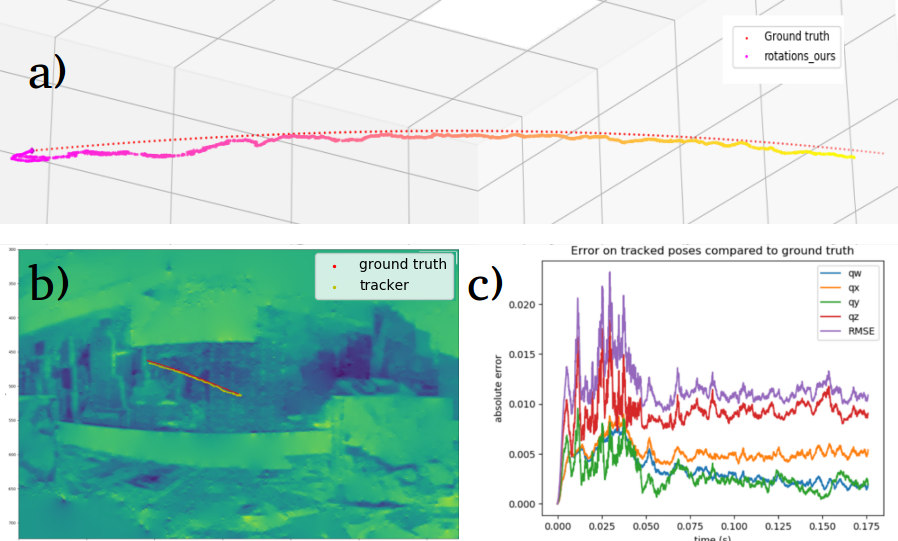
\includegraphics[width=1.0\linewidth]{figures/tracker_output.png}   
    \caption{Pose estimation on simulated dataset. \textbf{a:} Camera pose on unit sphere. Pink to yellow for tracked pose, red-dotted for ground truth. \textbf{b:} Tracked pose (yellow) and ground truth (red) overlaid on top of the reconstructed intensity map. \textbf{c:} Evaluation of the tracker algorithm. The absolute difference between the estimated poses and the ground truth is plotted against the time. The different quaternions qw, qx, qy, qz are plotted in blue, orange, green and red respectively. The RMSE (total pose error) is plotted in purple. }
    \label{fig:tracker_simulated}
\end{figure}

\subsubsection{Simultaneous Reconstruction and Tracking}
The algorithm proposed by Kim et al. \cite{kim2014simultaneous} bases on the assumption, that after each time step (or event batch, in our case), the reconstructing part and tracking part get a true value from each other. Since the tracker needs some initial time to localize itself and, doing so, performs a seemingly random walk in the beginning, the reconstruction part fails in our case and outputs a random B&W pattern. 



\subsection{Recorded Dataset}
For the recorded dataset, we intended to follow the same modular procedure as for the simulated dataset. 

\subsubsection{Mosaicing}
We based the reconstruction on the event stream and the inertial measurement unit (IMU) of the camera. \cref{fig:own_reconstruction} shows, that the dataset was not sufficiently good to return a successful reconstruction of the scene. 
\begin{figure}[h!]
	\centering
    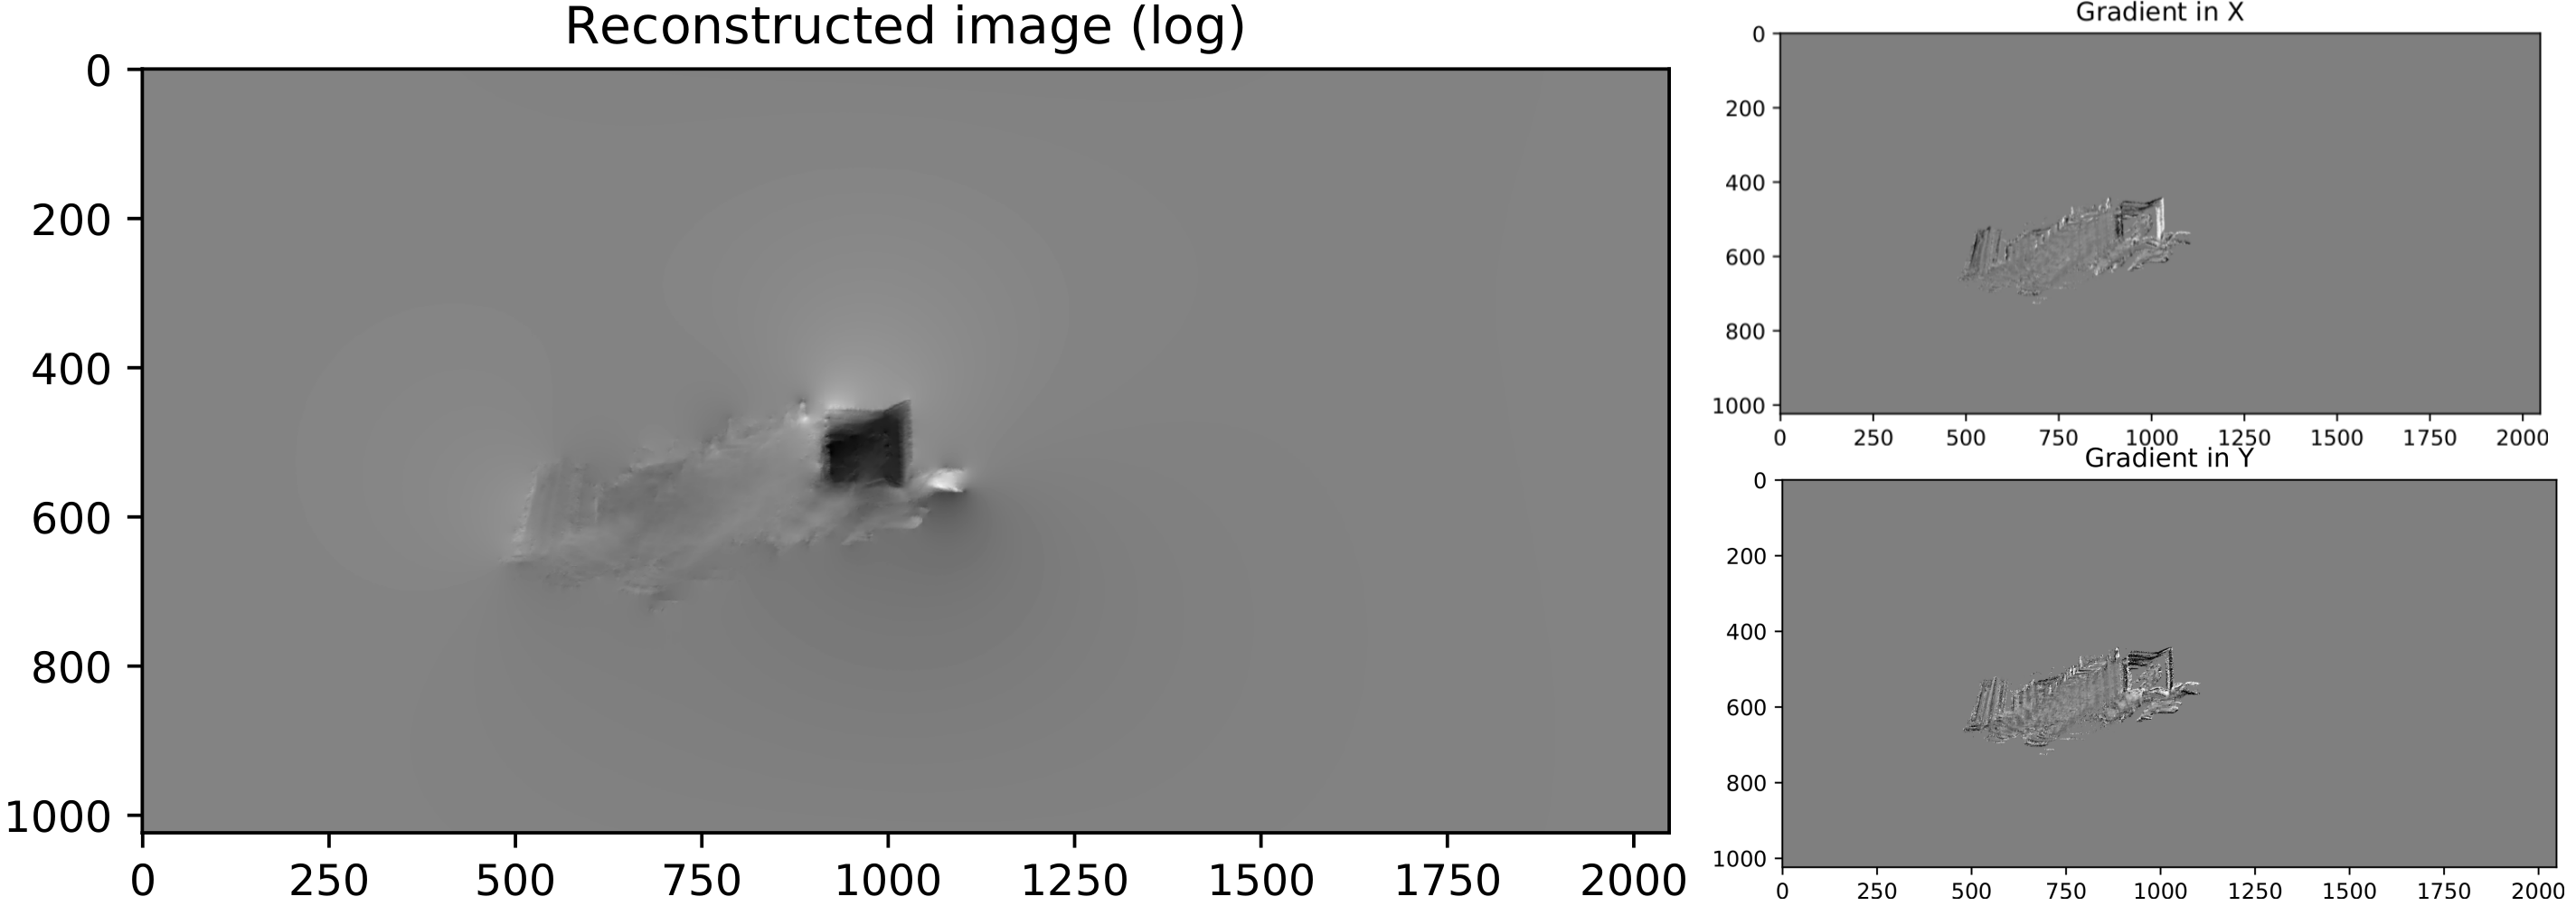
\includegraphics[width=1.0\linewidth]{figures/reconstruction_redroom.png}
    \caption{Reconstruction with own dataset. \textbf{left:} Reconstructed image of the simulated scene after Poisson solver is applied to gradient maps. \textbf{right:} Gradient maps in x and y respectively.}
    \label{fig:own_reconstruction}
\end{figure}

A investigation of the problem led us to conclude, that either the IMU is prone by errors or there is too much noise on the event stream. To tackle the first possibility, we tried to improve the ground truth poses by running the ORB-SLAM algorithm on the frames obtained from the APS of the camera. A screen shot of the procedure is shown in \cref{fig:orbslam}. 

\begin{figure}[h!]
	\centering
    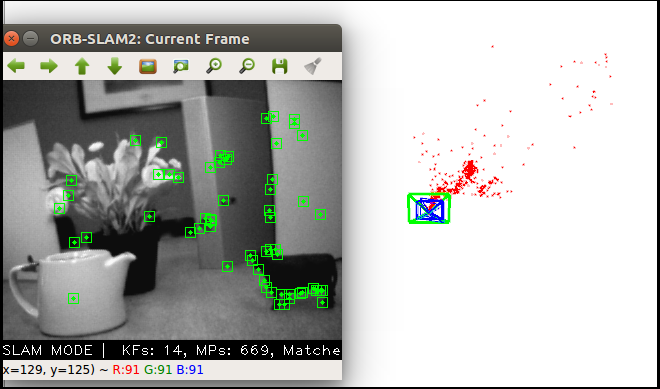
\includegraphics[width=1.0\linewidth]{figures/orbslam.png}
    \caption{ORB-SLAM algorithm applied to DAVIS frames. \textbf{left:} One frame with the tracked feature points (green) overlapped. \textbf{right:} Calculated camera pose and tracked feature points with respect to the virtual origin. }
    \label{fig:orbslam}
\end{figure}

Because the reconstruction algorithm is very susceptible to a low pose frequency, we adjusted the threshold for image generation in ORB-SLAM to return more poses per seconds. Thus, we could get a maximum of around ten poses per second, which is still a factor of 100 lower than the number of IMU data points of the camera. In order to run a successful intensity reconstruction based on an event stream, accurate poses are needed in steps in at least millisecond regime. Consequently, ORB-SLAM was not an appropriate approach to enhance the IMU data for an improved intensity reconstruction output. 

\subsubsection{Tracking}
Due to the lack of a reconstructed intensity map, we were not able to run the tracking algorithm on our recorded dataset. 

\subsection{Computational Effort}
Both parts of the algorithm, the mosaicing and the tracking part, rely on a sequential event stream. Thus, a parallelization is not possible without compromising accuracy in either of them. This leads to extremely long run times, which were exceeding several days even for relatively small data sets. The processing of several particles for the same event on the other hand can be done simultaneously. To implement this, we used Pandas\footnote{A data analysis toolkit based on Cython, see \url{https://pandas.pydata.org}} in those parts, which intrinsically is distributing the work load over the CPUs. This resulted in a significant speed-up of around 30\%. 


\section{Summary and Discussion}
In the scope of this project, we re-implement the tracking and mosaicing algorithms proposed by Kim et al. \cite{kim2014simultaneous} in Python. On the simulated, noise free data we achieved good performance on the mosaicing algorithm and acceptable results on the probabilistic tracking algorithm. We assume that the high complexity of the scene did force the tracker to perform bad in the initial stage and thus not allow an iterative approach of mosaicing and tracking. Thus, choosing a simpler scene could have been beneficial. 

Further, we applied the method to a dataset that we recorded with a DAVIS348. The reconstruction algorithm was not successful; although some prominent features are recognizable, there are no details visible. We assumed the problem to be a bad IMU accuracy and tackled it by applying ORB-SLAM to the APS frames and thus obtaining better poses. However, due to the low rate of generated poses per second, this did not improve the output of the algorithm. Without a reconstructed scene, the tracking was not possible for the recorded dataset. 

Additionally we figured, that the sequential nature of the algorithm results in a very long run time, thus running the tracker for a full rotation is not feasible within a few hours. 

\subsection{Next steps}
Continuing this work, we summarize some possible next steps to take. 

In order to connect the two parts of the algorithm in order to replicate the result of \cite{kim2014simultaneous}, we would choose a dataset with less complexity, assuming that the tracker would work better on such. In order to do so it would be highly beneficial to optimize the run time, thus one could think of implementing the code in C++ instead of Python. Also the question arises if the computationally expensive Particle Filtering is the best approach. Looking at the results of a follow-up paper \cite{kim2} supports this: By choosing C++  and replacing the Particle Filter with an Extended Kalman Filter, Kim et al. report on implementing the simultaneous tracking and mapping in real-time.

Moreover we think, that the algorithm should be optimized to work on noisy datasets. A possible method could include a non-linear Bayesian approach as in \cite{paperpresentation} where the likelihood function for the events takes noise into account and thus is more resilient to outliers. 

One suggestion of obtaining a dataset with correct reference poses is to mount the event camera on a mechanical rotating arm with controlled and tracked motion. 

\section{Our Work}

\subsection{Our Contribution}

Firstly, we implemented a mosaicing and tracking algorithms for event cameras based on the theoretical framework of \cite{kim2014simultaneous} in Python. As per our research, no other open-source Particle Filter based tracking algorithm exists for an event-based camera.
Moreover, we re-implemented the open-source reconstruction code from Guillermo Gallego in Python. 
Lastly, we generated a new dataset with a DAVIS, that includes ground truth poses. These are improved by applying ORB-SLAM to the RGB stream.

\subsection{Work Distribution}
All authors worked on literature research , that included a meeting with Guillermo Gallego, author of \cite{EventVisionReview} and \cite{reinbacher}.
Nik Dennler implemented the intensity reconstruction algorithm. All Authors contributed to the Particle Filter and helped in generating a new dataset. C\'eline Nauer and Nik Dennler applied ORB-SLAM to this data. All authors worked on the write-up of this report.

\newpage

{\small
\bibliographystyle{unsrt}
\bibliographystyle{ieee}
\bibliography{egbib}
}

\end{document}
